% Source: graduate-coursework/Research/Intro_to_Agents/handouts/Part5_TwoLayer_Agents.tex

\documentclass[border=4pt]{standalone}
\usepackage[T1]{fontenc}
\usepackage{graphicx}
\usepackage{lmodern}
\usepackage{tikz}
\usepackage{xcolor}
\usetikzlibrary{shapes.geometric, arrows.meta, positioning, fit, calc, backgrounds}

\definecolor{UofSCGarnet}{HTML}{73000a}
\definecolor{UofSCBlack}{HTML}{000000}
\definecolor{UofSCWhite}{HTML}{ffffff}
\definecolor{UofSCRose}{HTML}{CC2E40}
\definecolor{UofSCAtlantic}{HTML}{466A9F}
\definecolor{UofSCCongaree}{HTML}{1F414D}
\definecolor{UofSCHorseshoe}{HTML}{65780B}
\definecolor{UofSCGrass}{HTML}{CED318}
\definecolor{UofSCHoneycomb}{HTML}{A49137}
\definecolor{UofSC90Black}{HTML}{363636}
\definecolor{UofSC70Black}{HTML}{5C5C5C}
\definecolor{UofSC50Black}{HTML}{A2A2A2}
\definecolor{UofSCWarmGrey}{HTML}{676156}
\definecolor{UofSCSandstorm}{HTML}{FFF2E3}
\definecolor{UofSCDarkGarnet}{HTML}{570008}
\definecolor{UofSCAzalea}{HTML}{844247}

\tikzset{
    % Box styles - all sharp corners
    orchestrator/.style={
        rectangle,
        draw=UofSCGarnet,
        fill=UofSCGarnet!10,
        line width=1.5pt,
        minimum width=4cm,
        minimum height=1.2cm,
        align=center,
        font=\bfseries
    },
    worker/.style={
        rectangle,
        draw=UofSCAtlantic,
        fill=UofSCAtlantic!10,
        line width=1pt,
        minimum width=2cm,
        minimum height=0.9cm,
        align=center
    },
    task/.style={
        rectangle,
        draw=UofSCCongaree,
        fill=UofSCCongaree!10,
        line width=1pt,
        minimum width=1.8cm,
        minimum height=0.8cm,
        align=center
    },
    process/.style={
        rectangle,
        draw=UofSCBlack,
        fill=UofSCWhite,
        line width=1pt,
        minimum width=3cm,
        minimum height=0.8cm,
        align=center
    },
    result/.style={
        rectangle,
        draw=UofSCHorseshoe,
        fill=UofSCHorseshoe!10,
        line width=1pt,
        minimum width=2.5cm,
        minimum height=0.8cm,
        align=center
    },
    decision/.style={
        diamond,
        draw=UofSCGarnet,
        fill=UofSCGarnet!10,
        line width=1pt,
        minimum width=2cm,
        minimum height=1cm,
        align=center,
        aspect=2
    },
    % Arrow styles - straight lines only
    arrow/.style={
        ->,
        >=Stealth,
        line width=1pt,
        draw=UofSCBlack
    },
    thickarrow/.style={
        ->,
        >=Stealth,
        line width=1.5pt,
        draw=UofSCGarnet
    },
    dashedarrow/.style={
        ->,
        >=Stealth,
        line width=1pt,
        draw=UofSC70Black,
        dashed
    }
}

\begin{document}
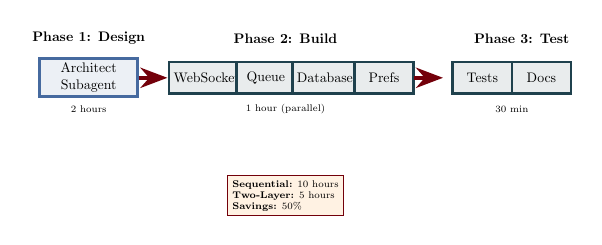
\begin{tikzpicture}[scale=0.5, transform shape]
    % Phase 1
    \node[font=\bfseries] at (-5,3.5) {Phase 1: Design};
    \node[worker, minimum width=2.5cm] (arch) at (-5,2.5) {Architect\\Subagent};
    \node[font=\scriptsize] at (-5,1.7) {2 hours};

    % Phase 2
    \node[font=\bfseries] at (0,3.5) {Phase 2: Build};
    \node[task, minimum width=1.5cm] (c1) at (-2,2.5) {WebSocket};
    \node[task, minimum width=1.5cm] (c2) at (-0.5,2.5) {Queue};
    \node[task, minimum width=1.5cm] (c3) at (1,2.5) {Database};
    \node[task, minimum width=1.5cm] (c4) at (2.5,2.5) {Prefs};
    \node[font=\scriptsize] at (0,1.7) {1 hour (parallel)};

    % Phase 3
    \node[font=\bfseries] at (6,3.5) {Phase 3: Test};
    \node[task, minimum width=1.5cm] (d1) at (5,2.5) {Tests};
    \node[task, minimum width=1.5cm] (d2) at (6.5,2.5) {Docs};
    \node[font=\scriptsize] at (5.75,1.7) {30 min};

    % Arrows
    \draw[thickarrow] (arch) -- (-3,2.5);
    \draw[thickarrow] (c4) -- (4,2.5);

    % Timeline comparison
    \node[draw=UofSCGarnet, fill=UofSCSandstorm, align=left, font=\scriptsize] at (0,-0.5) {
        \textbf{Sequential:} 10 hours\\
        \textbf{Two-Layer:} 5 hours\\
        \textbf{Savings:} 50\%
    };
\end{tikzpicture}
\end{document}
